\documentclass{article}

\usepackage{fullpage}
\usepackage{graphicx}

\title{Homework 4}
\author{Caius Brindescu \and Mihai Codoban \and Semih Okur \and Shao Yuan \and Kyungho Leoo}

\begin{document}

\maketitle

\begin{figure}
	\begin{center}
		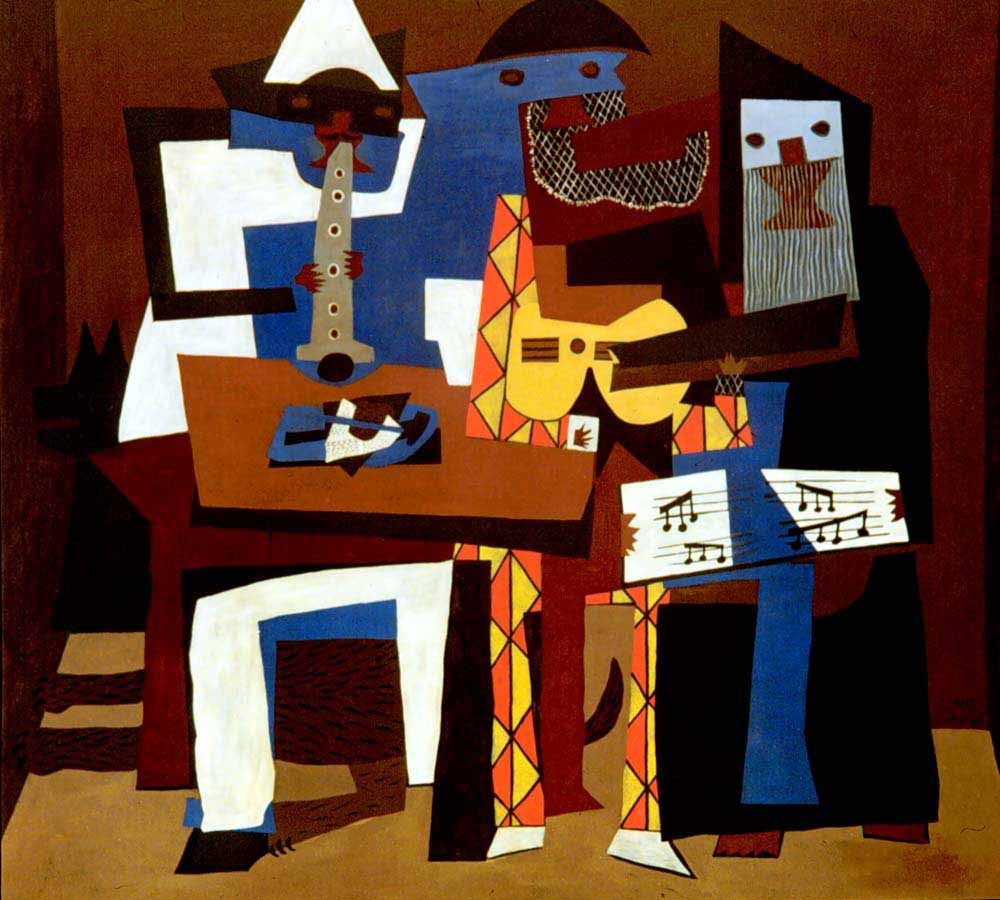
\includegraphics{image.jpg}
	\end{center}
	\caption{The image we used}
	\label{fig:image}
\end{figure}

\begin{figure}
	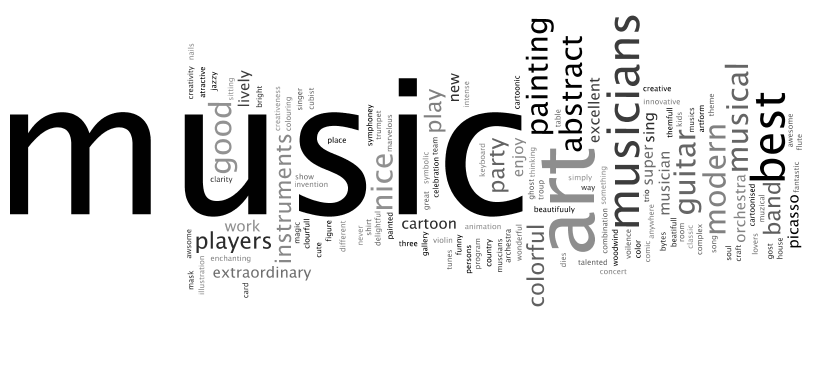
\includegraphics[width=\textwidth]{wordcloud.png}
	\caption{The word cloud}
	\label{fig:cloud}
\end{figure}

\begin{enumerate}

\item What programming environment did you use? What did you use for generating the word cloud?

We used Java and Eclipse for interacting with the Mechanical Turk and Python for generating the word cloud.

\item Where did the visual design come from and why did you choose it?

\item How many workers were involved in producing the final word cloud?

50.

\item What was the total labor cost for producing the word cloud? Don't include the costs related to any earlier experimentation.

\$1.00

\item How long did it take to produce the word cloud (i.e. from the time the program was started to when the word cloud was returned)?

If this includes the time it took for the tasks to be completed, about  a day. If it refers only for the time needed to compute the word cloud, then it was less than 1 second.

\item Diagram the overall workflow or process that you implemented to produce the word cloud.

\item How would you characterize the quality of the first impressions captured by the word cloud?

\item How did the first impressions returned by the crowd match or deviate from your group's expectations for the design?

Since it was an abstract piece of art, we did not have particular expectations. Wer

\item Describe some ways that might improve the efficiency or outcomes of the task? For example, how could you achieve a higher quality outcome; or how could you reduce the number of workers required, the total labor costs, or the time required to produce an outcome of the same quality?

\item From the perspective of the designer who created the design used in the project, how might being able to collect first impressions from potential users benefit the design process?

\end{enumerate}

\end{document}